\documentclass{article}
\usepackage{graphicx} % Required for inserting images
\usepackage{subcaption}
\usepackage{placeins} % Added to use \FloatBarrier and control image placement
\usepackage{float}    % Added for advanced float positioning [H]
\usepackage{hyperref} % Good practice for cross-referencing


\usepackage{biblatex}
\addbibresource{references.bib}

\title{SU compmath module 1 - Ecology}
\author{Felix Almay\\
Onyinyechi Sonia Bäckström\\
Matilda Colarieti Tosti}
\date{\today}

\begin{document}

\maketitle
\newpage

\section{Introduction}

This report looks at two closely related butterflies: \textit{Pieris rapae} (the small white, known in Sweden as \textit{rovfjäril}) and \textit{Pieris napi} (the green-veined white, or \textit{rapsfjäril}). Both species are bivoltine, meaning they produce two generations per year: a spring generation that emerges from overwintered pupae, and a subsequent summer generation that develops from eggs laid by the spring generation adults \cite{british_lepidoptera_rapae} \cite{british_lepidoptera_napi}. Both species are very common in Sweden and other parts of the world. Because they are so closely related, they behave in very similar ways. However, by looking closely at when they fly during the year and where they are found in different parts of the country, we can see how they have adapted differently to their environments.

\section{Methods}

Observation data for \textit{Pieris rapae} and \textit{Pieris napi} were retrieved from Artportalen \cite{artportalen} as two tab-separated value (TSV) files. We chose to restrict the data to the years 2000-2025, excluding 2026 for the statistical analyses (figures \ref{fig:seasonal_phenology}, \ref{fig:latitude_effect}, \ref{fig:latitude-species},\ref{fig:climate_trend}) as full data for this year is not yet available. 

% Note that the histograms include partial data from 2026, and that findings for which the time period exceeds one week are not included in the histograms.

The artificial intelligence tool Gemini Notebook \cite{gemini_notebook} was utilized to implement and debug the analysis code, generate \LaTeX~code for the report and in some cases formulate the authors' ideas regarding the results as draft report text for the discussion section.

The programming language Python 3 \cite{python3} was used for the analysis code. 

Code quality assurance and formatting were conducted using the static analysis tool Pylint \cite{pylint}.

\newpage

\section{Results}

% \begin{figure}[!htb]
%     \centering
%     \begin{subfigure}[b]{0.49\linewidth}
%         \centering
%         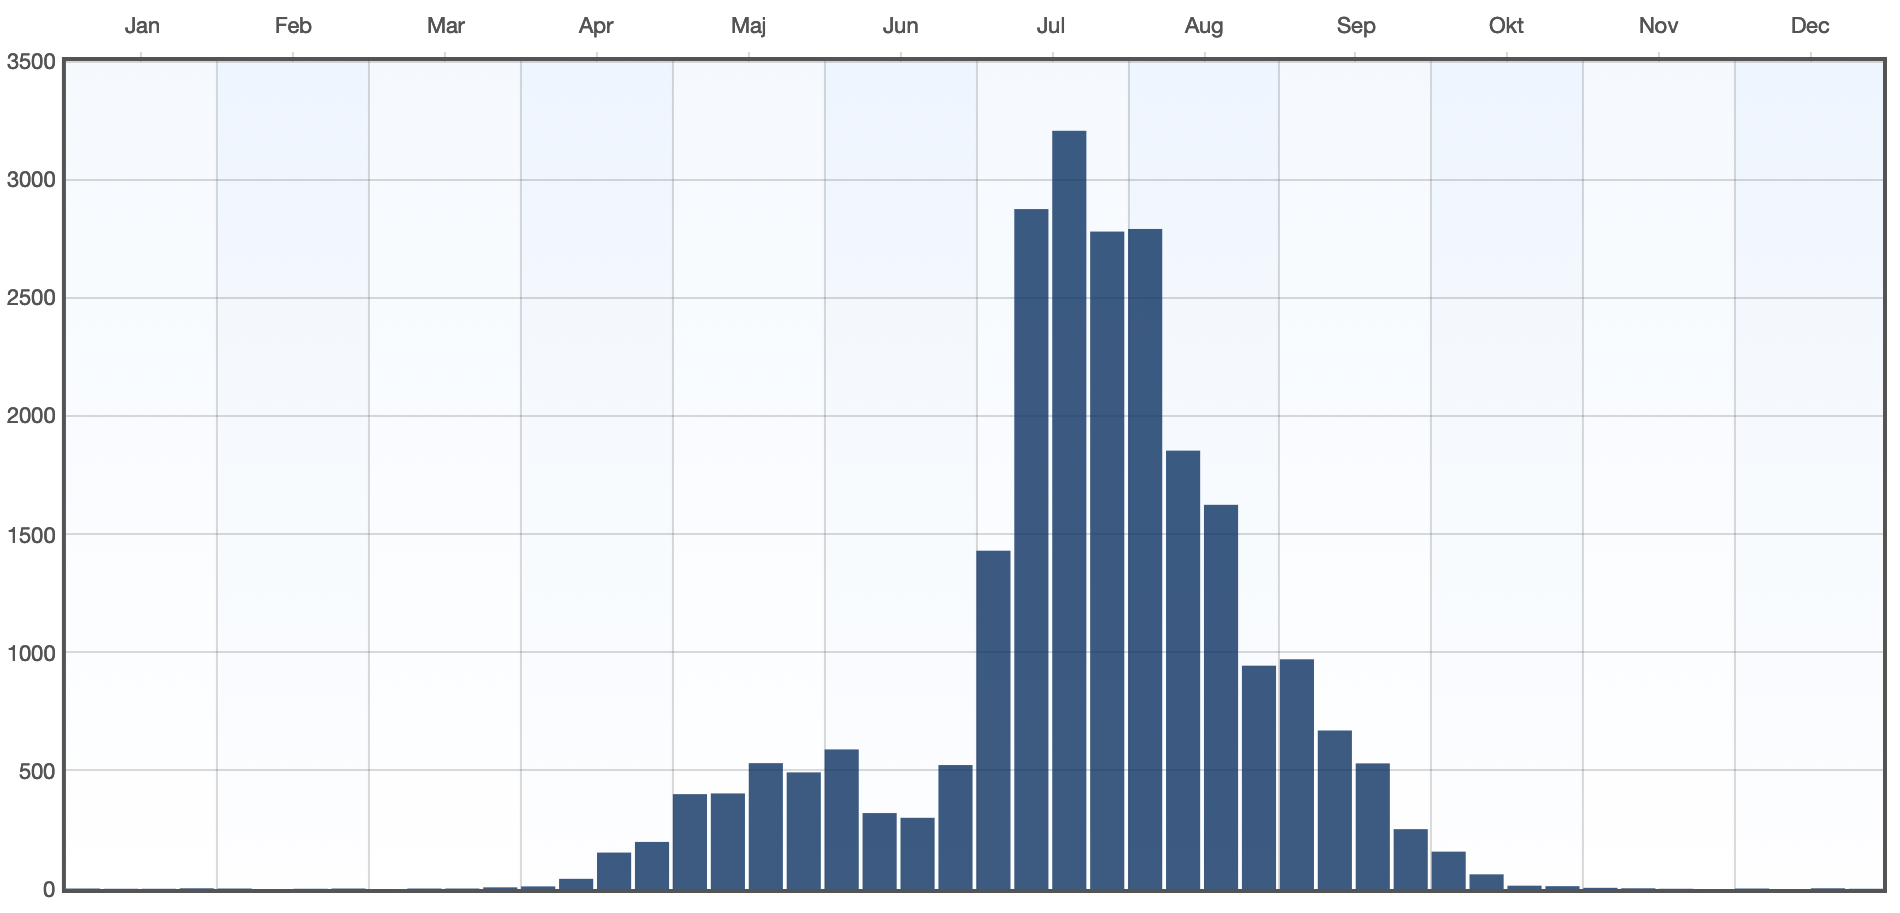
\includegraphics[width=\linewidth]{figures/ROV.wholesweden.week.png}
%         \caption{Small White (\textit{Pieris rapae})}
%         \label{fig:rovfjari}
%     \end{subfigure}
%     \hfill
%     \begin{subfigure}[b]{0.49\linewidth}
%         \centering
%         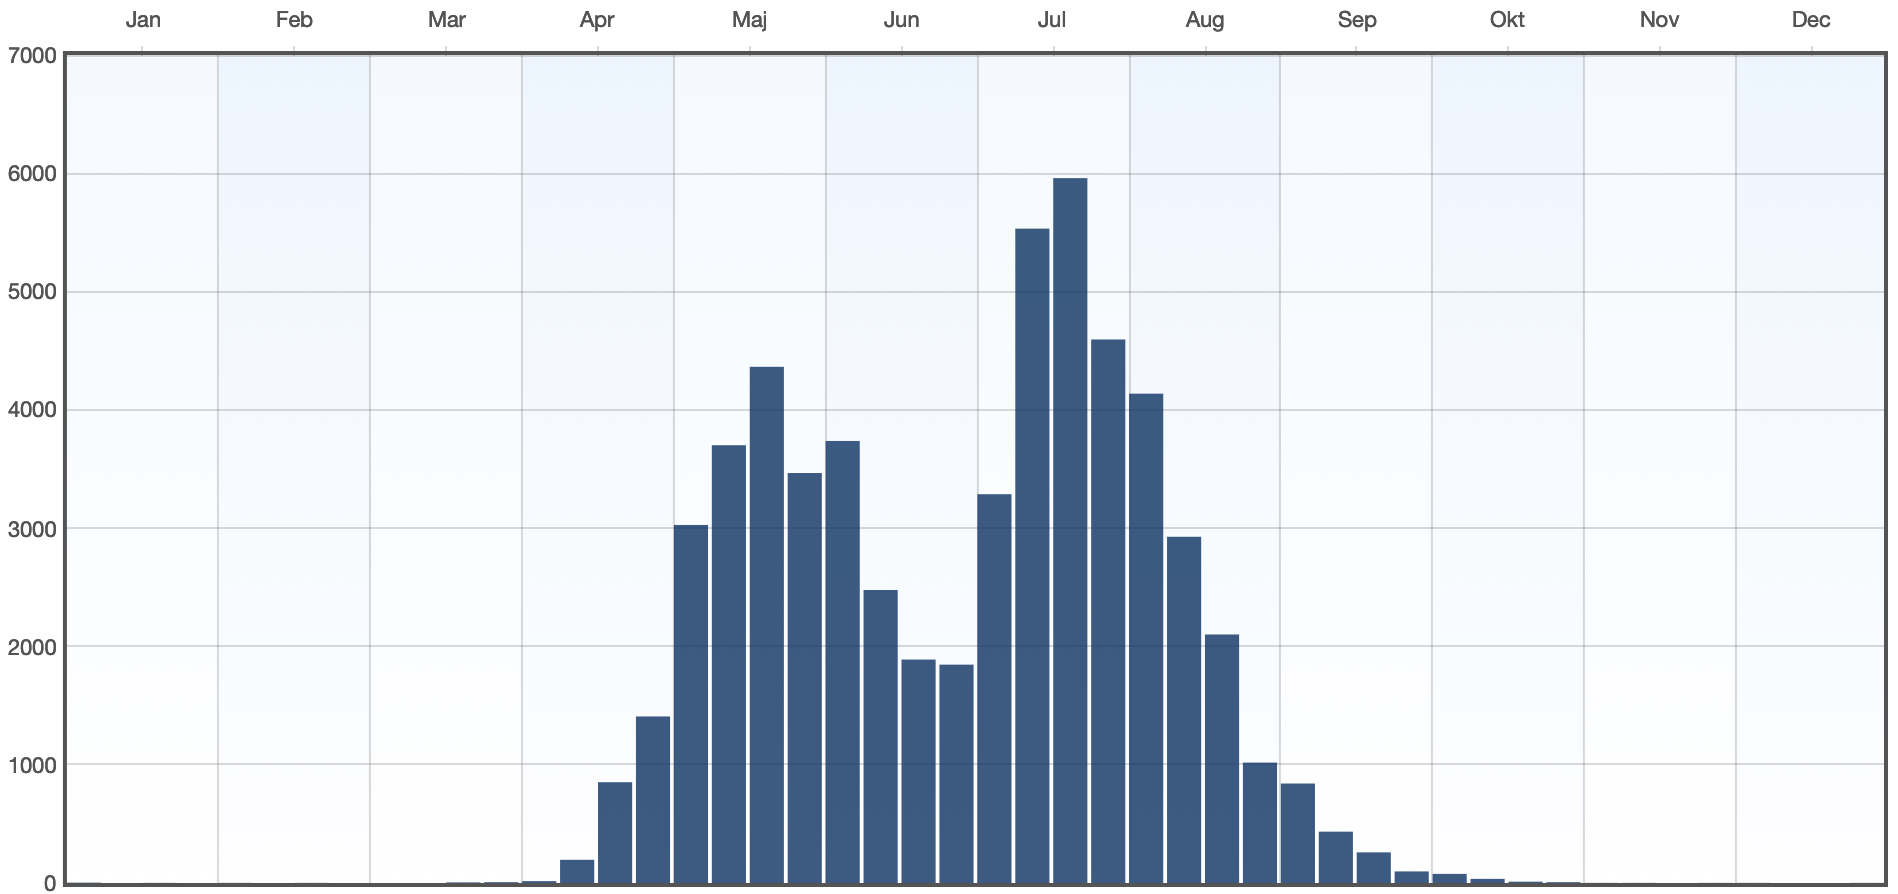
\includegraphics[width=\linewidth]{figures/RAPS.wholesweden.week.png}
%         \caption{Green-veined White (\textit{Pieris napi})}
%         \label{fig:rapsfjari}
%     \end{subfigure}
%     \caption{Weekly observation frequency of the two butterfly species in Sweden from 2000 to 2026. Both species show a two-generation seasonal pattern, but they differ significantly in total volume and spring activity.}
%     \label{fig:butterfly_comparison}
% \end{figure}

% \begin{figure}[!htb]
%     \centering
%     \begin{subfigure}[t]{0.48\linewidth}
%         \centering
%         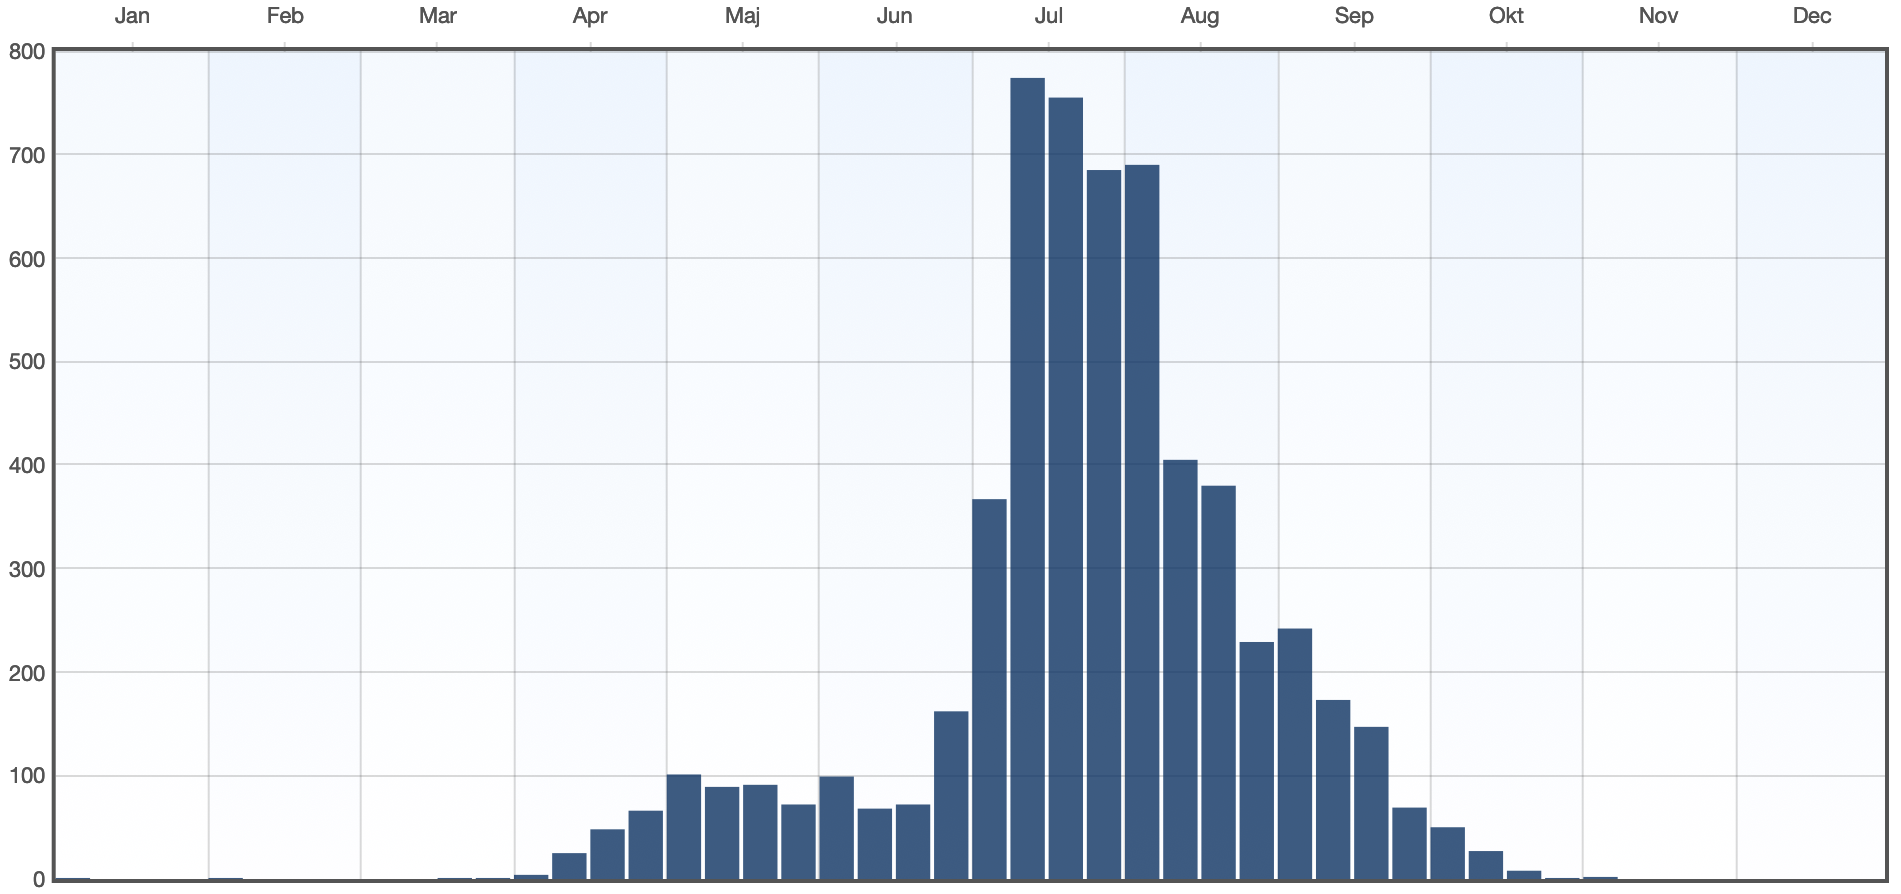
\includegraphics[height=5cm, width=\linewidth, keepaspectratio]{figures/ROV.south.week.png}%
%         \caption{Small White (\textit{Pieris rapae}) in Southern Sweden}
%         \label{fig:rov_south}
%     \end{subfigure}% <-- Förhindrar radbrytning
%     \hfill%
%     \begin{subfigure}[t]{0.48\linewidth}
%         \centering
%         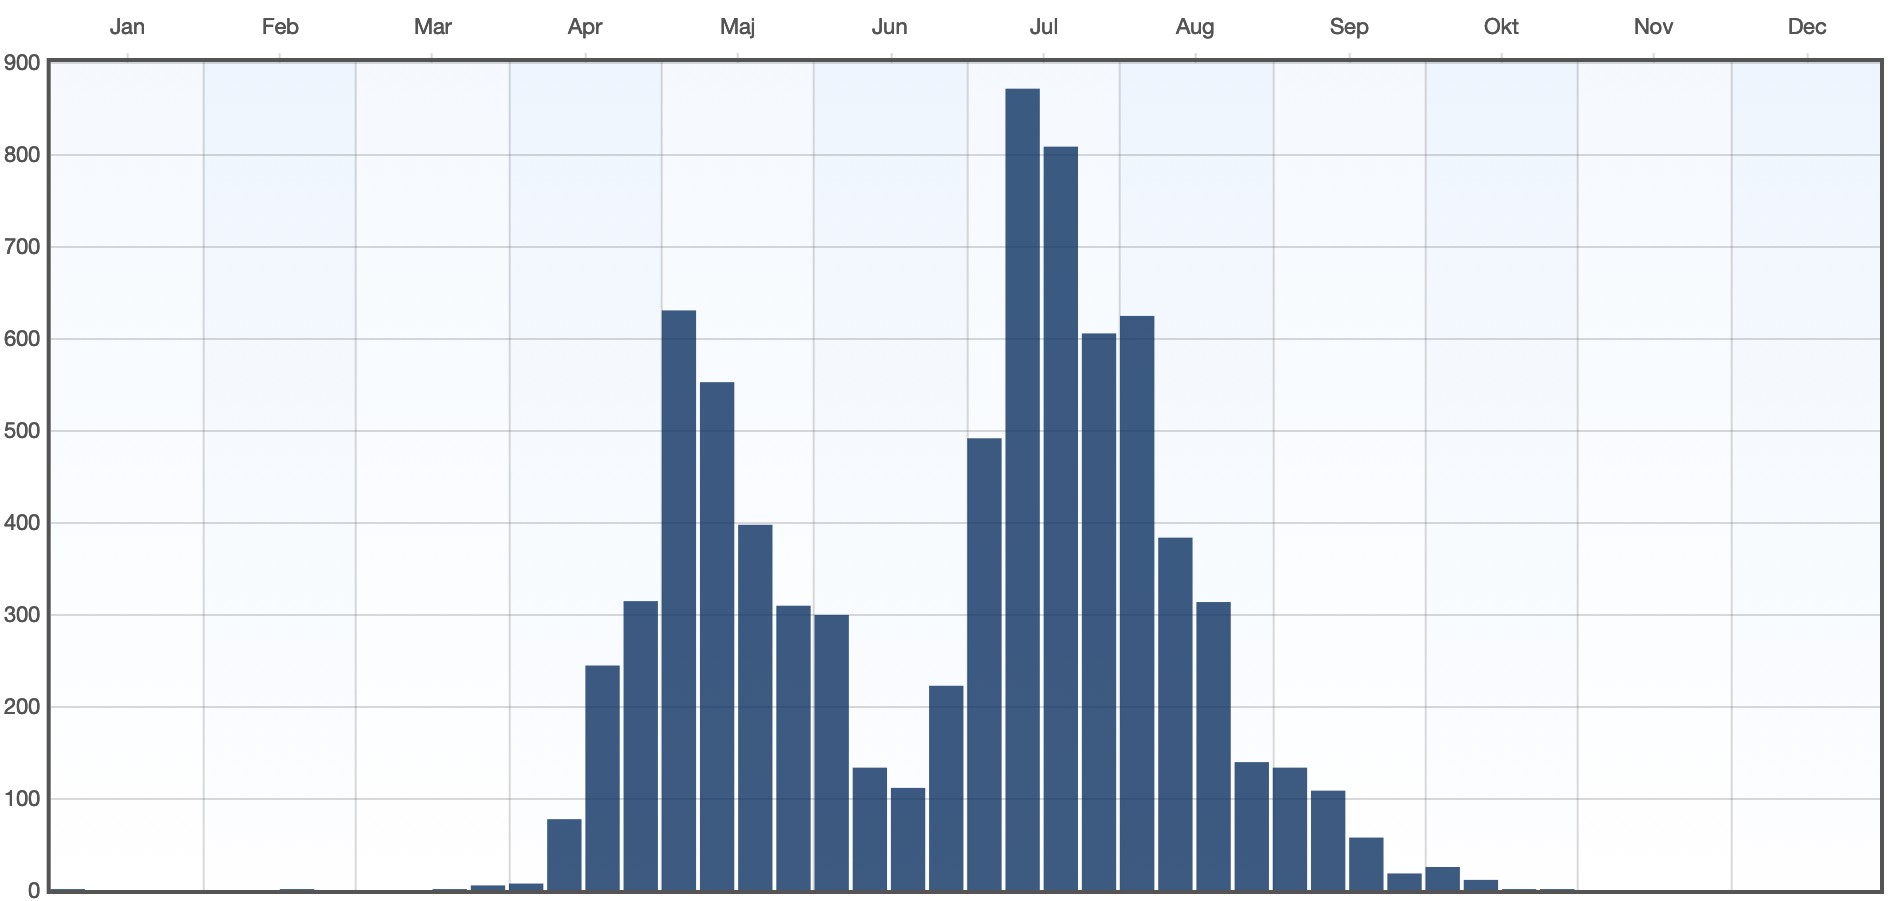
\includegraphics[height=5cm, width=\linewidth, keepaspectratio]{figures/RAPS.south.week.png}%
%         \caption{Green-veined White (\textit{Pieris napi}) in Southern Sweden}
%         \label{fig:raps_south}
%     \end{subfigure}
%     \caption{Weekly observation frequency of the Small White and the Green-veined White in Southern Sweden (Scania) from 2000 to 2026. Both species show a clear two-generational lifecycle, though they differ in their spring and summer ratios.}
%     \label{fig:south_comparison}
% \end{figure}

% \begin{figure}[!htb]
%     \centering
%     \begin{subfigure}[t]{0.48\linewidth}
%         \centering
%         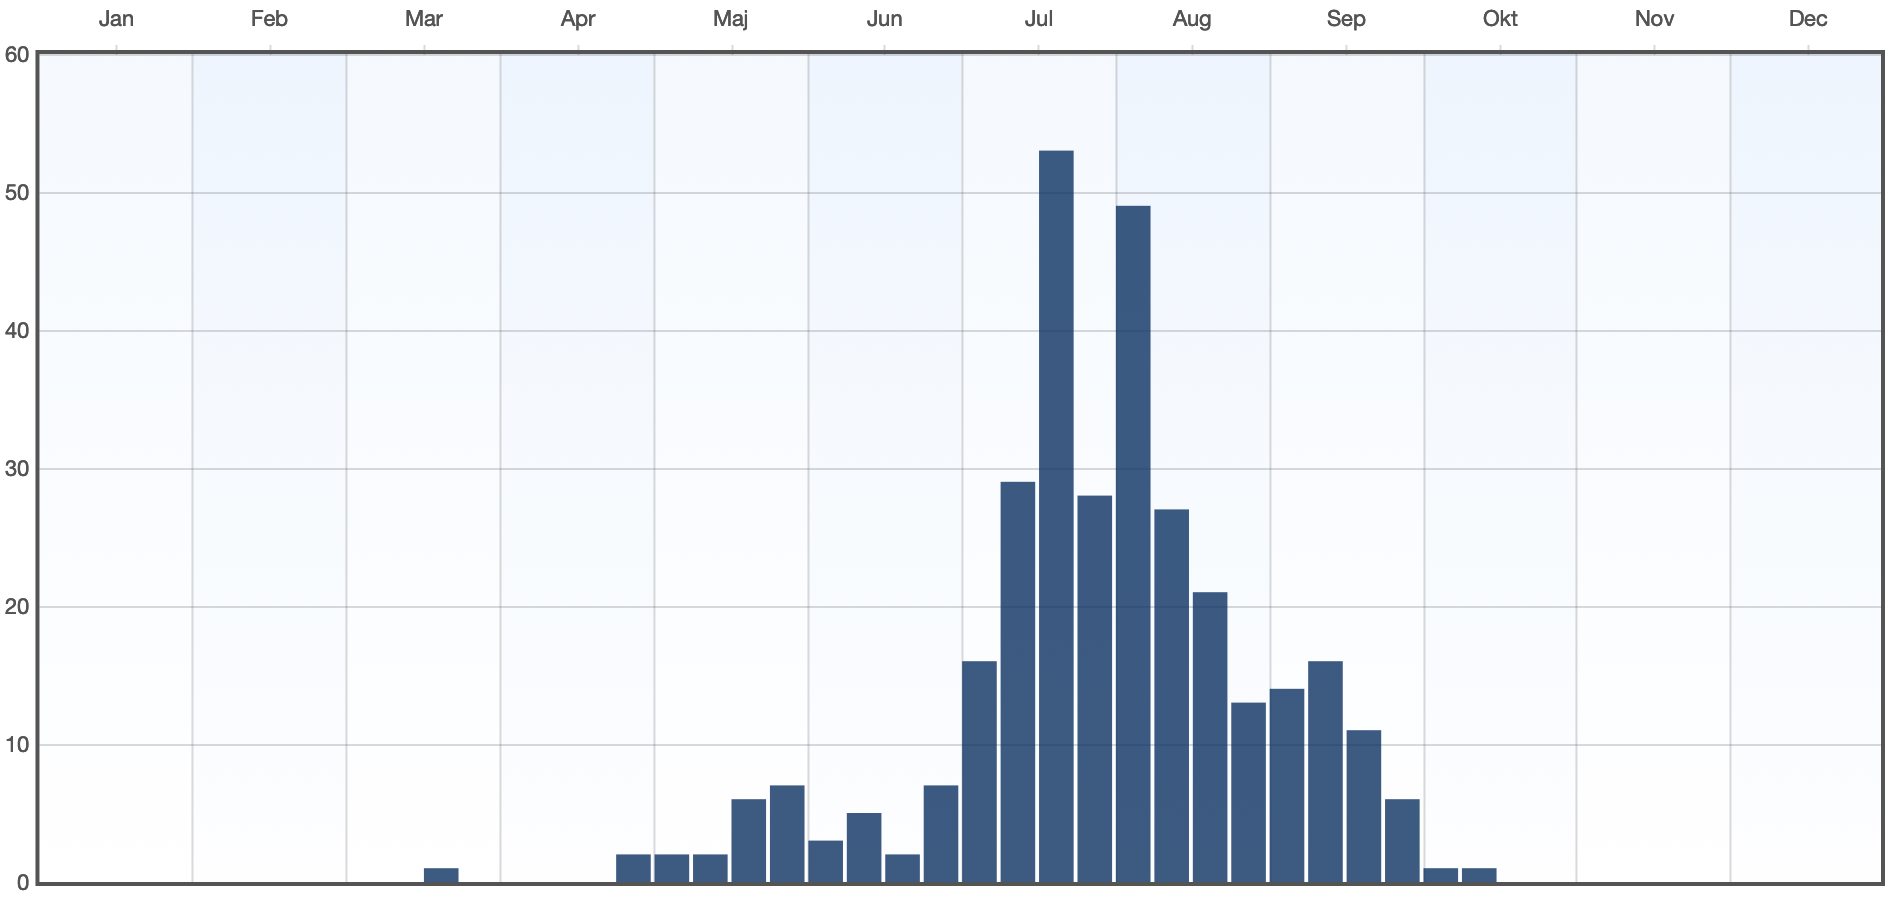
\includegraphics[height=5cm, width=\linewidth, keepaspectratio]{figures/ROV.middle.week.png}%
%         \caption{Small White (\textit{Pieris rapae}) in Middle Sweden}
%         \label{fig:rov_middle}
%     \end{subfigure}% <-- Förhindrar radbrytning
%     \hfill%
%     \begin{subfigure}[t]{0.48\linewidth}
%         \centering
%         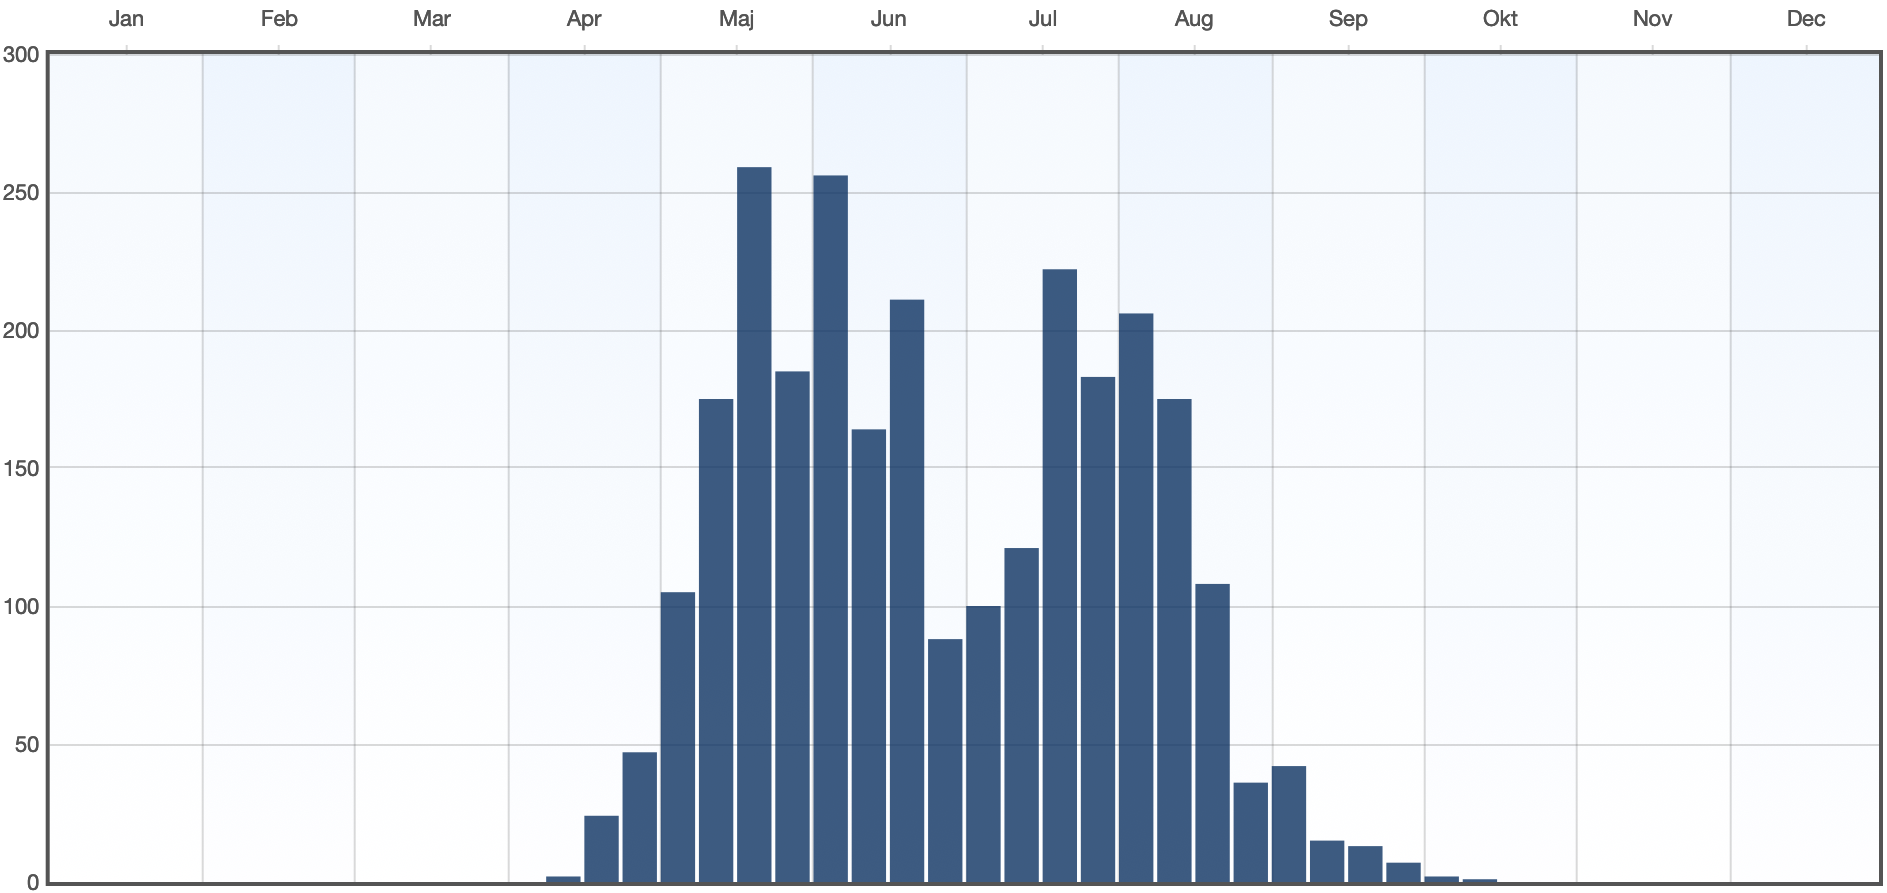
\includegraphics[height=5cm, width=\linewidth, keepaspectratio]{figures/RAPS.middle.week.png}%
%         \caption{Green-veined White (\textit{Pieris napi}) in Middle Sweden}
%         \label{fig:raps_middle}
%     \end{subfigure}
%     \caption{Weekly observation frequency of the Small White and the Green-veined White in Middle Sweden (Gävleborg and Dalarna) from 2000 to 2026. We note a heavily reduced abundance and near-absence of spring activity for the Small White.}
%     \label{fig:middle_comparison}
% \end{figure}

% \begin{figure}[!htb]
%     \centering
%     \begin{subfigure}[t]{0.48\linewidth}
%         \centering
%         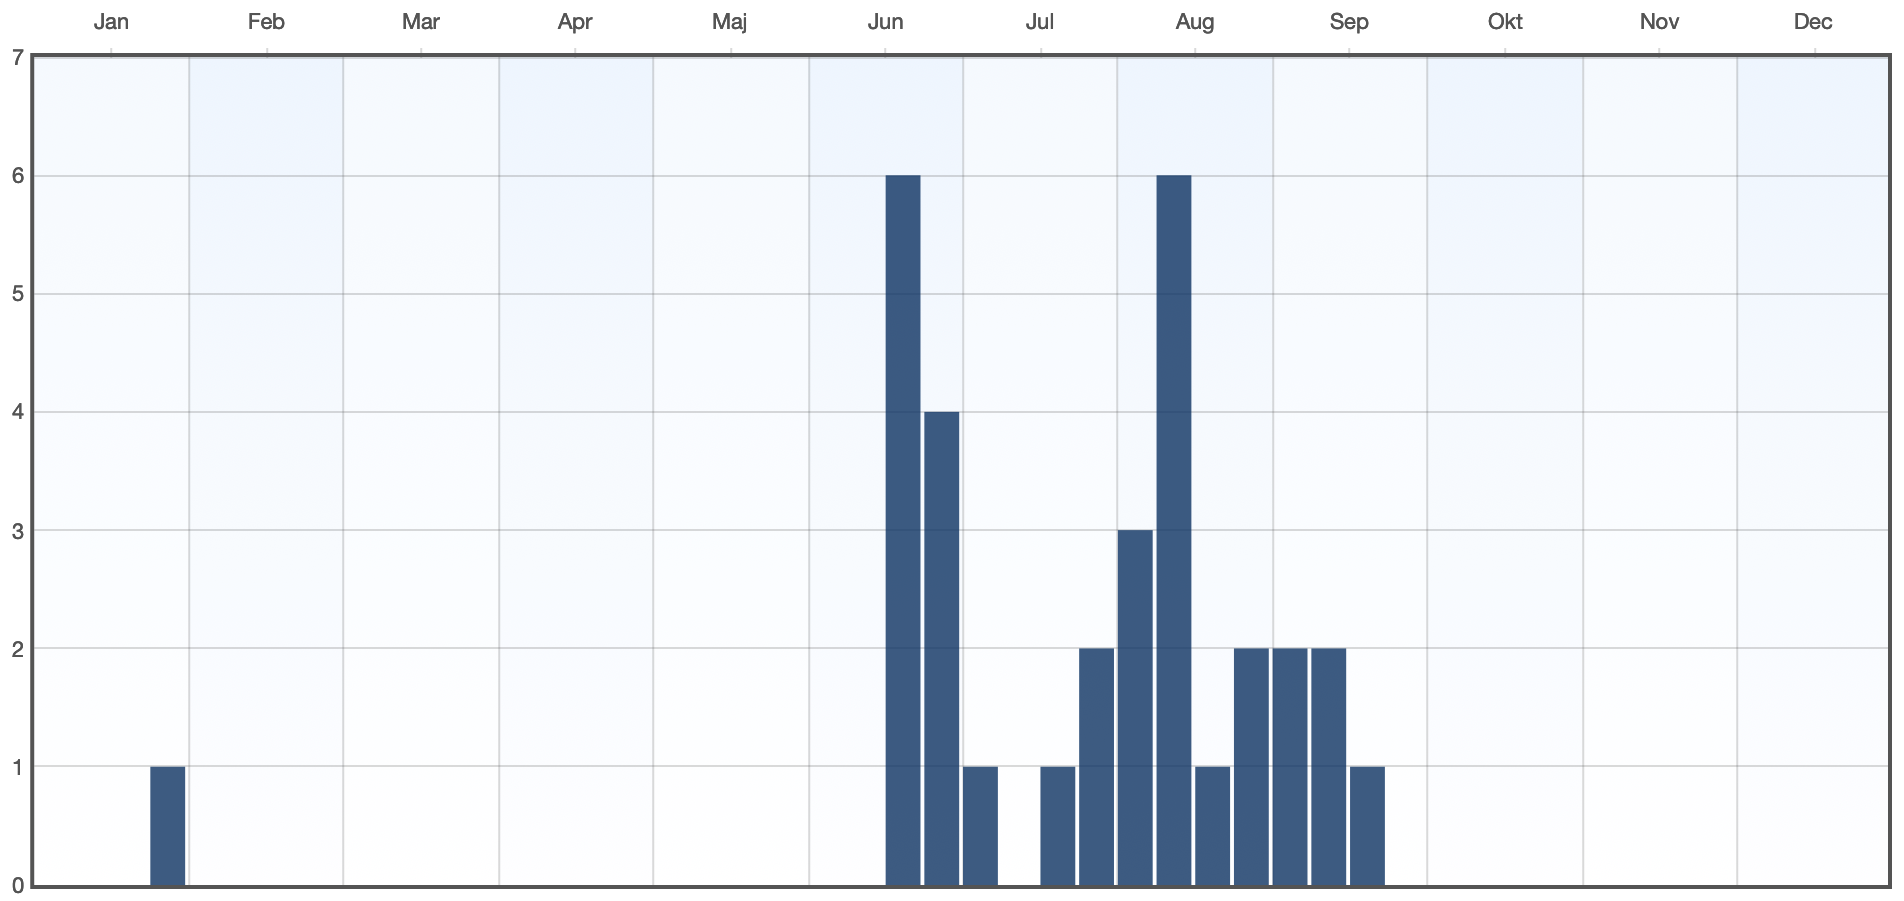
\includegraphics[height=5cm, width=\linewidth, keepaspectratio]{figures/ROV.north.week.png}%
%         \caption{Small White (\textit{Pieris rapae}) in Northern Sweden}
%         \label{fig:rov_north}
%     \end{subfigure}% <-- Förhindrar radbrytning
%     \hfill%
%     \begin{subfigure}[t]{0.48\linewidth}
%         \centering
%         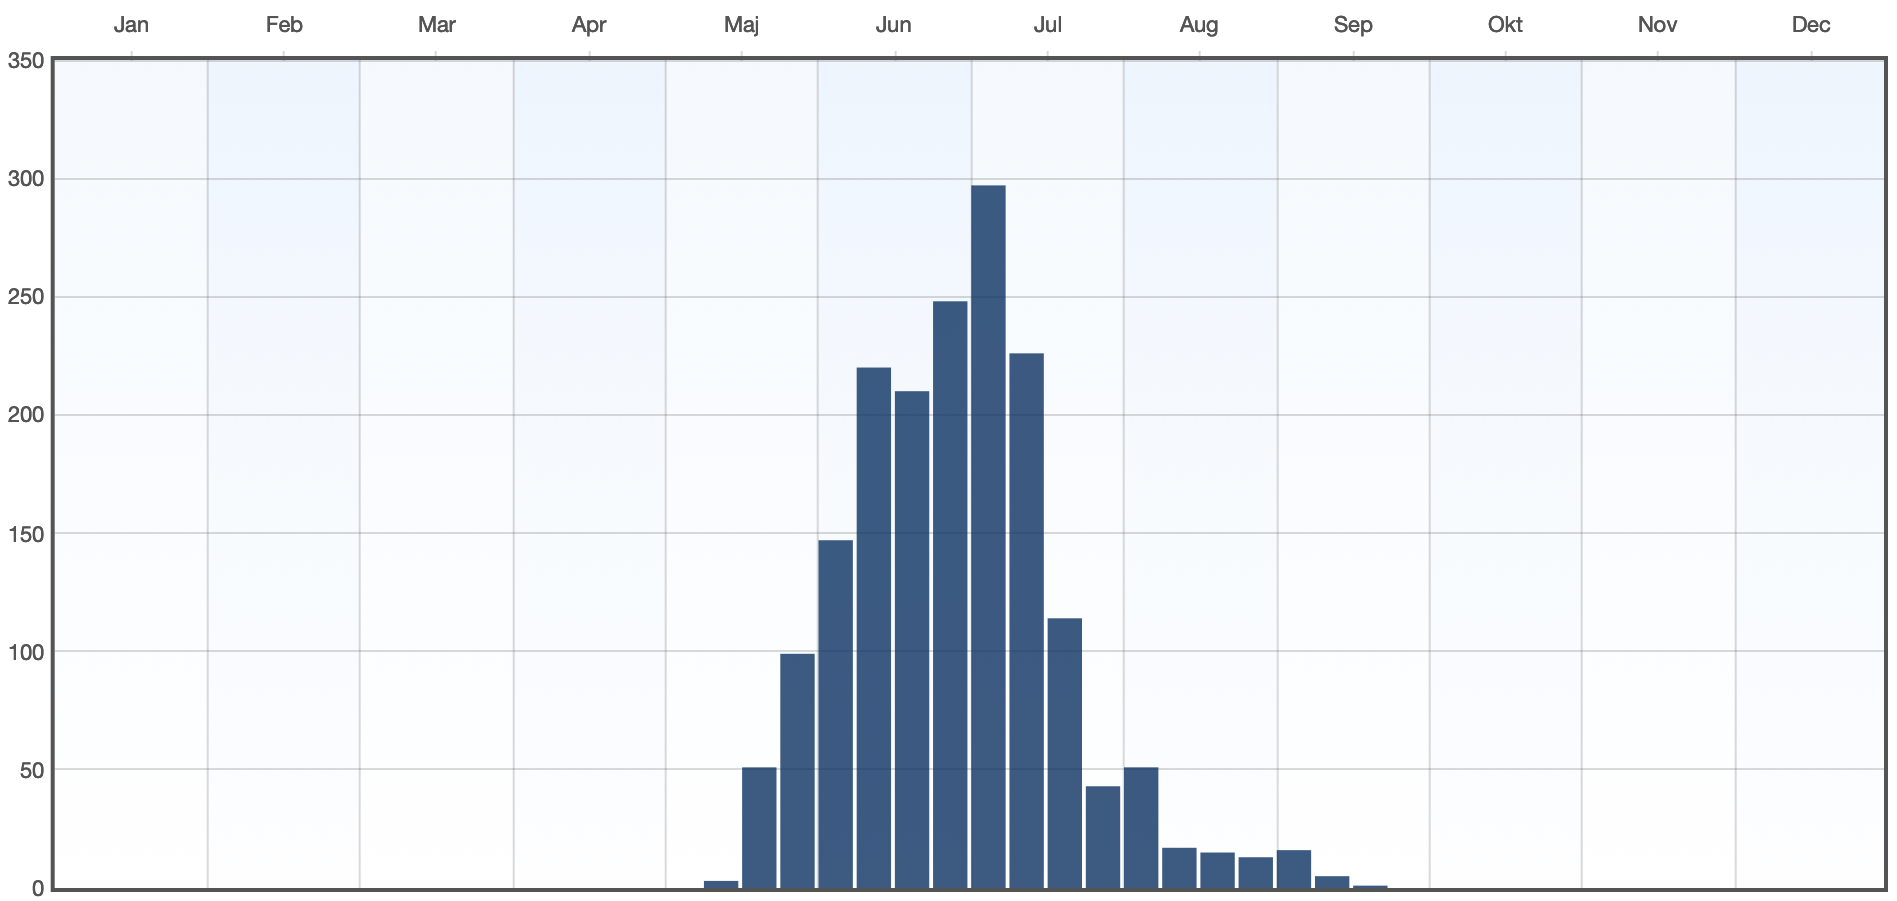
\includegraphics[height=5cm, width=\linewidth, keepaspectratio]{figures/RAPS.north.week.png}%
%         \caption{Green-veined White (\textit{Pieris napi}) in Northern Sweden}
%         \label{fig:raps_north}
%     \end{subfigure}
%     \caption{Weekly observation frequency of the Small White and the Green-veined White in Northern Sweden (Norrbotten) from 2000 to 2026. The Green-veined White transitions to a single, sharp summer generation, while the Small White is exceptionally rare.}
%     \label{fig:north_comparison}
% \end{figure}

\begin{figure}[!htb]
    \centering
    \makebox[\textwidth][c]{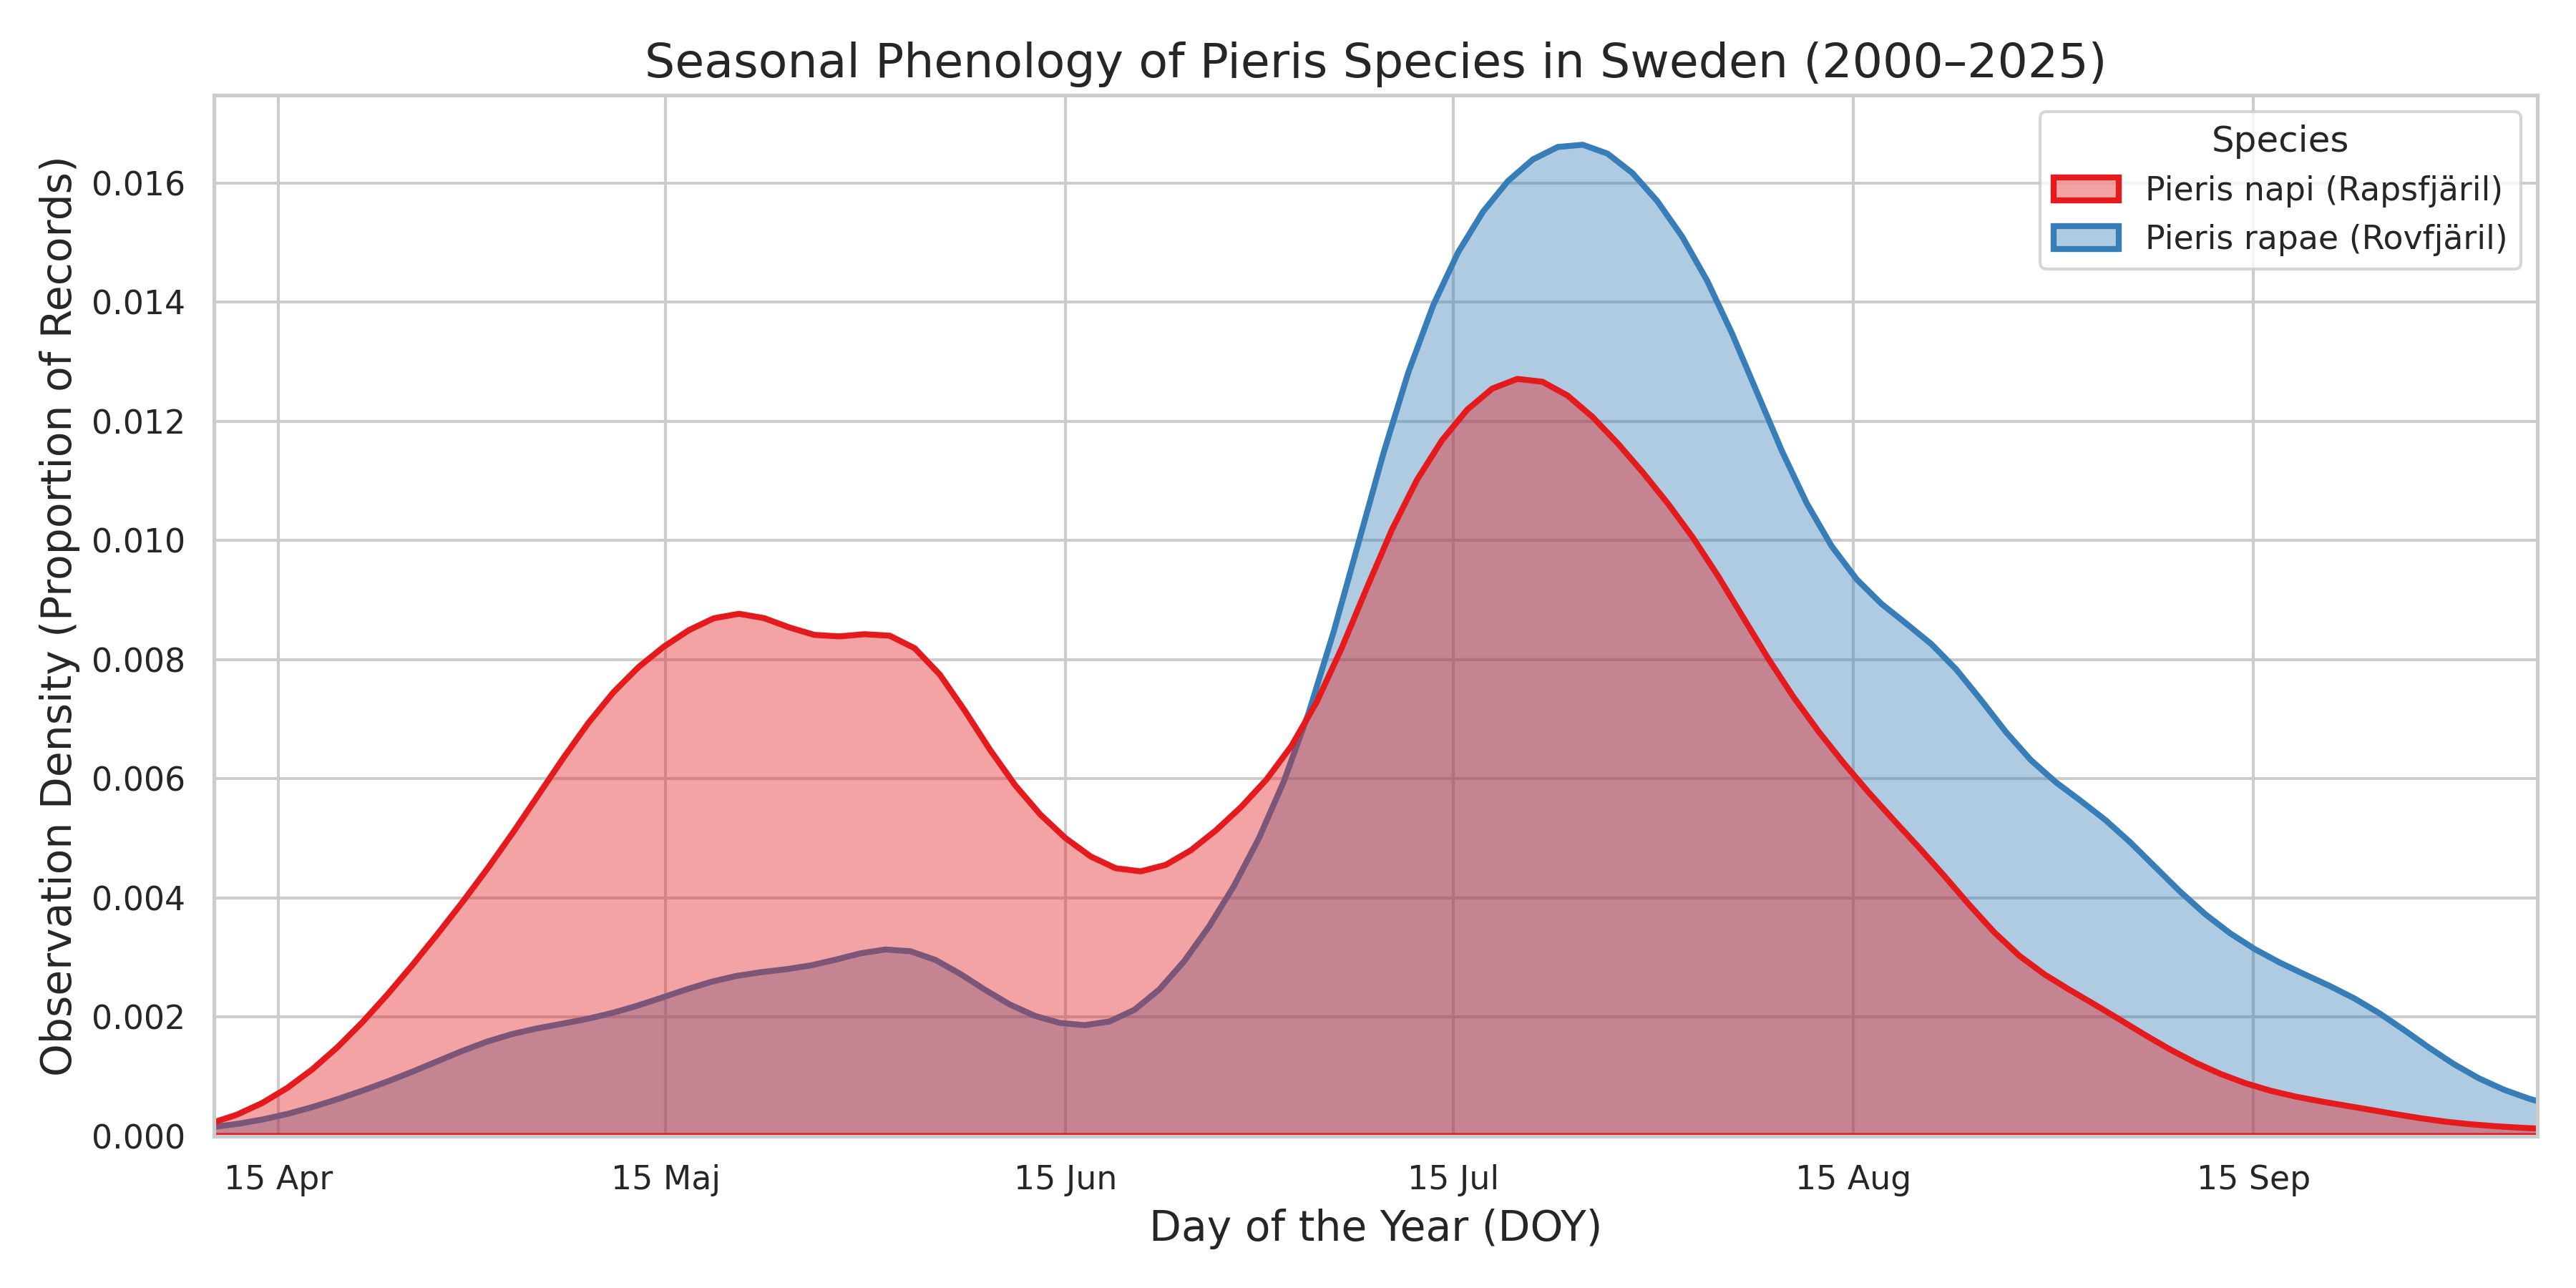
\includegraphics[width=1.15\textwidth]{figures/figure_1_seasonal_phenology.png}}
    \caption{Seasonal flight phenology of Pieris napi (green-veined white) and Pieris rapae (small white) in Sweden compiled from citizen science data (2000–2025). The Kernel Density Estimate (KDE) curves illustrate the temporal distribution of adult observations across the day of the year (DOY). Curves are independently normalized to show the relative proportion of records within each species.}
    \label{fig:seasonal_phenology}
\end{figure}

\begin{figure}[!htb]
    \centering
    \makebox[\textwidth][c]{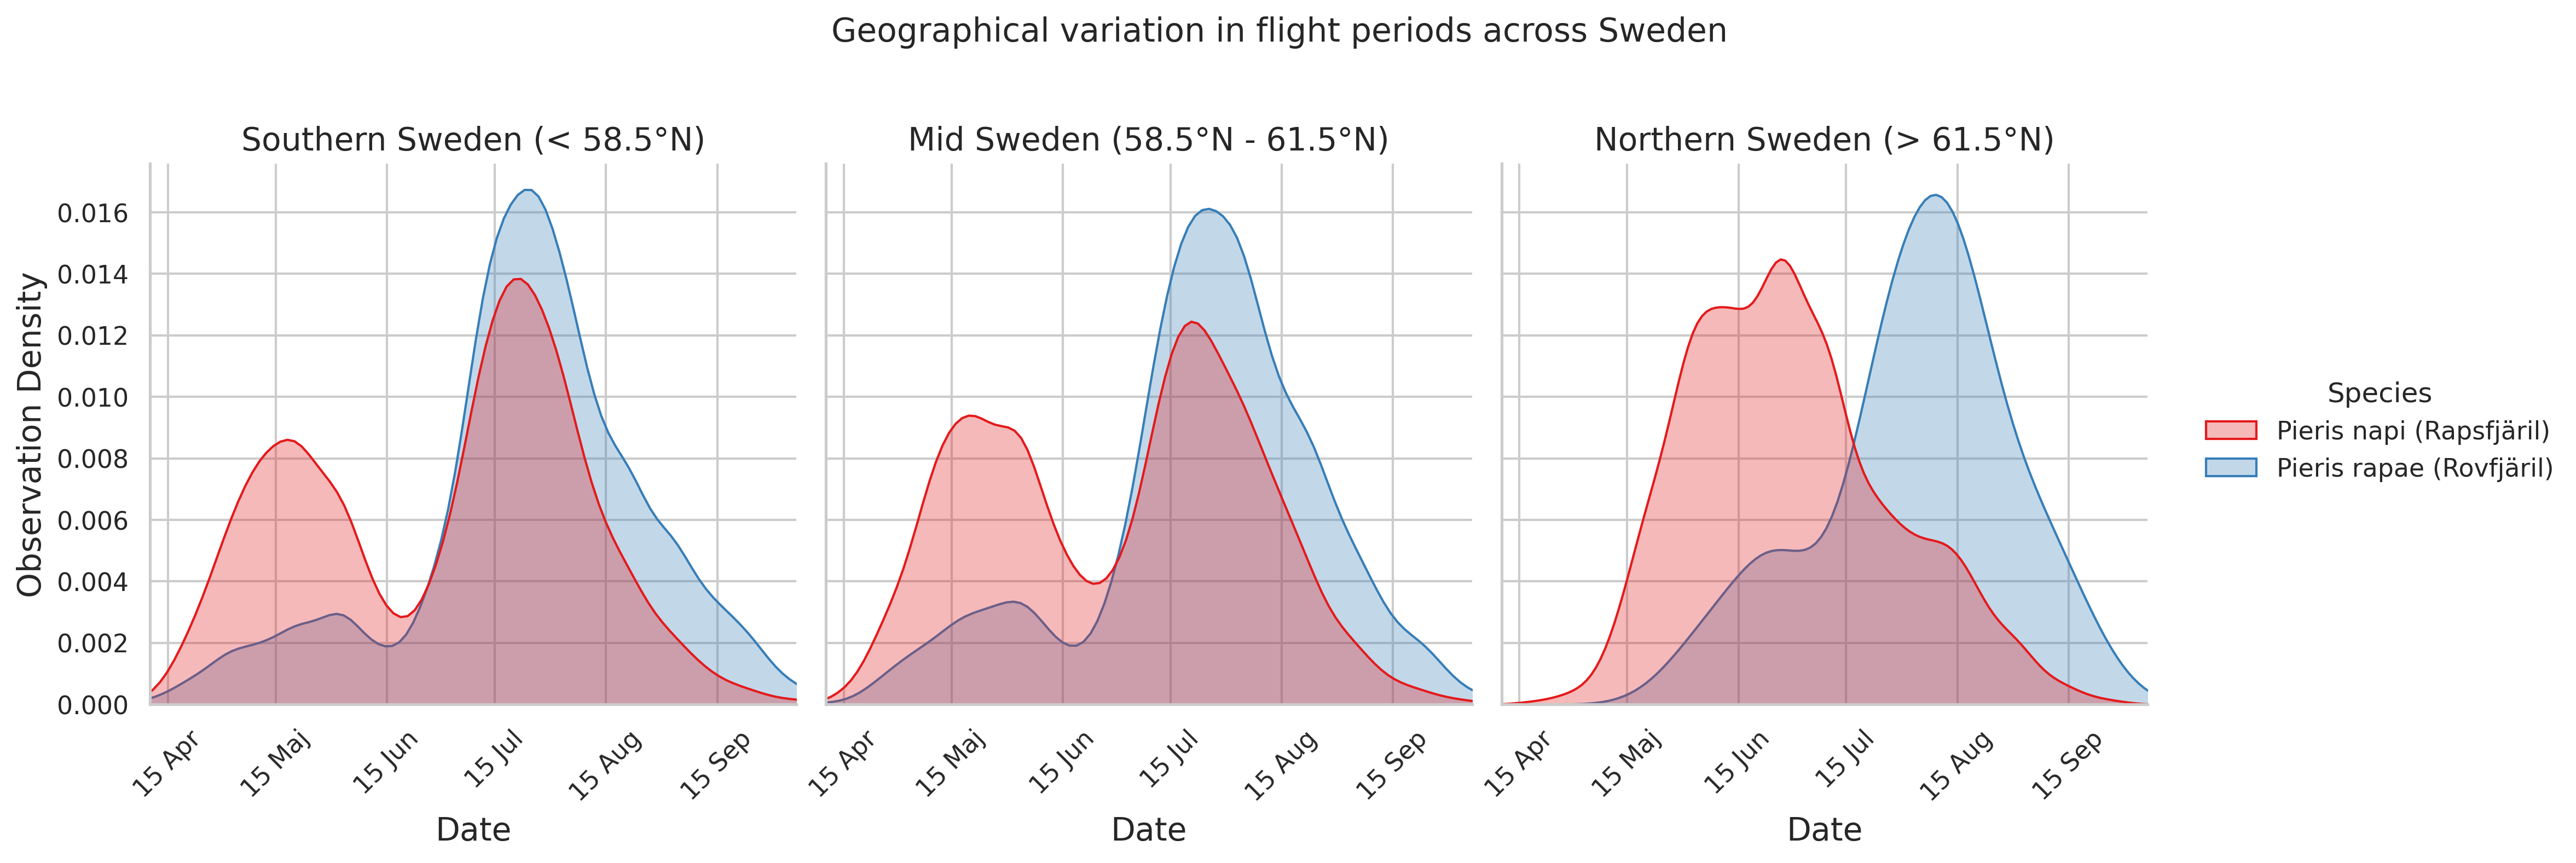
\includegraphics[width=1.4\textwidth]{figures/figure_2_latitude_effect.png}}
    \caption{Geographical variation in adult Pieris flight phenology across Sweden (2000–2025). Observations are partitioned into three latitudinal zones: Southern Sweden ($< 58.5^{\circ}$N), Mid Sweden ($58.5^{\circ}$N – $61.5^{\circ}$N), and Northern Sweden ($> 61.5^{\circ}$N).}
    \label{fig:latitude_effect}
\end{figure}

\begin{figure}[!htb]
    \centering
    
    \makebox[\textwidth][c]{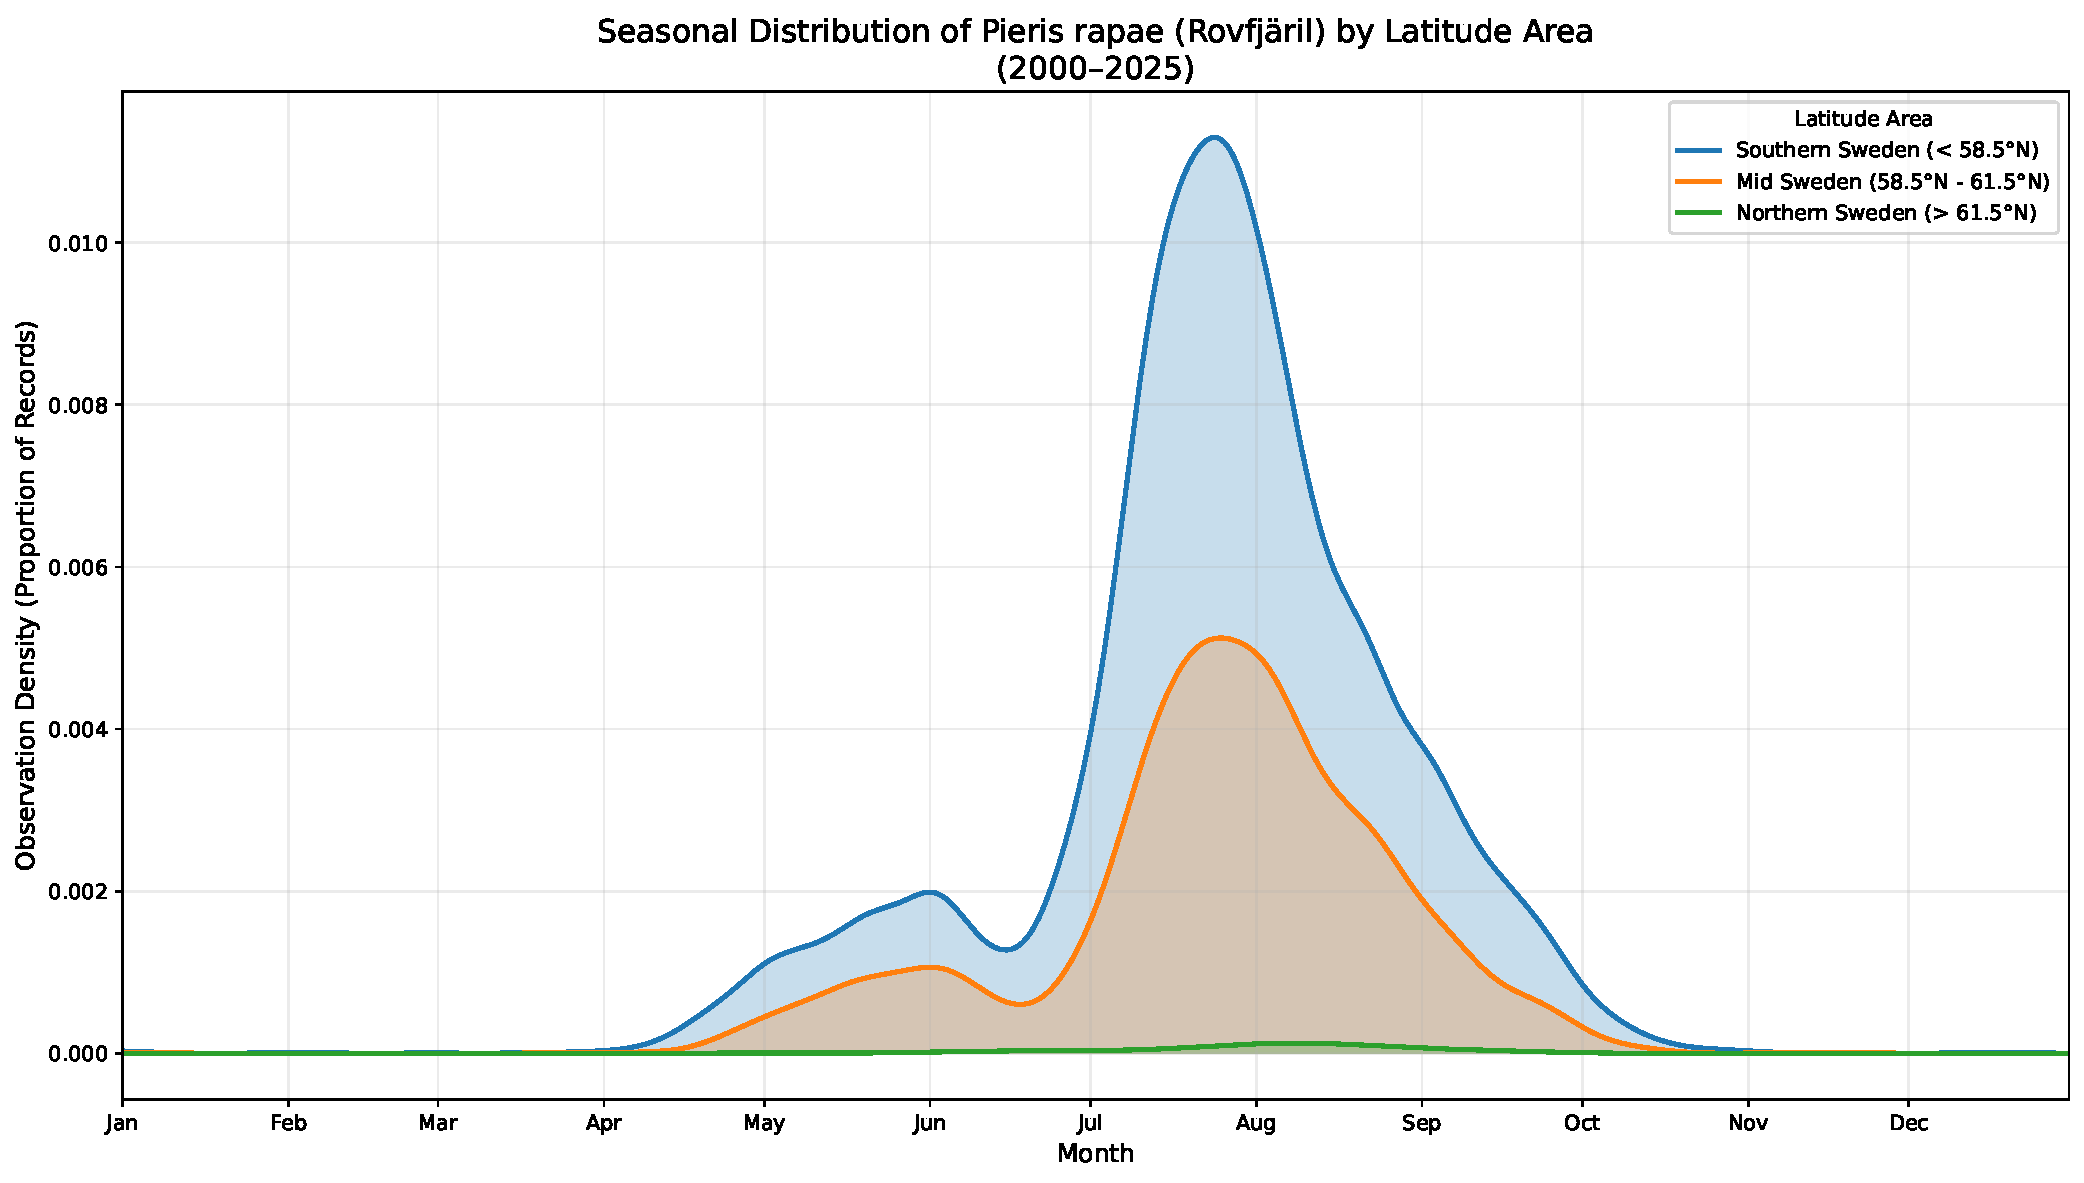
\includegraphics[width=1.3\textwidth]{figures/Pieris_rapae_latitude_density.pdf}}
    \hfill
    \makebox[\textwidth][c]{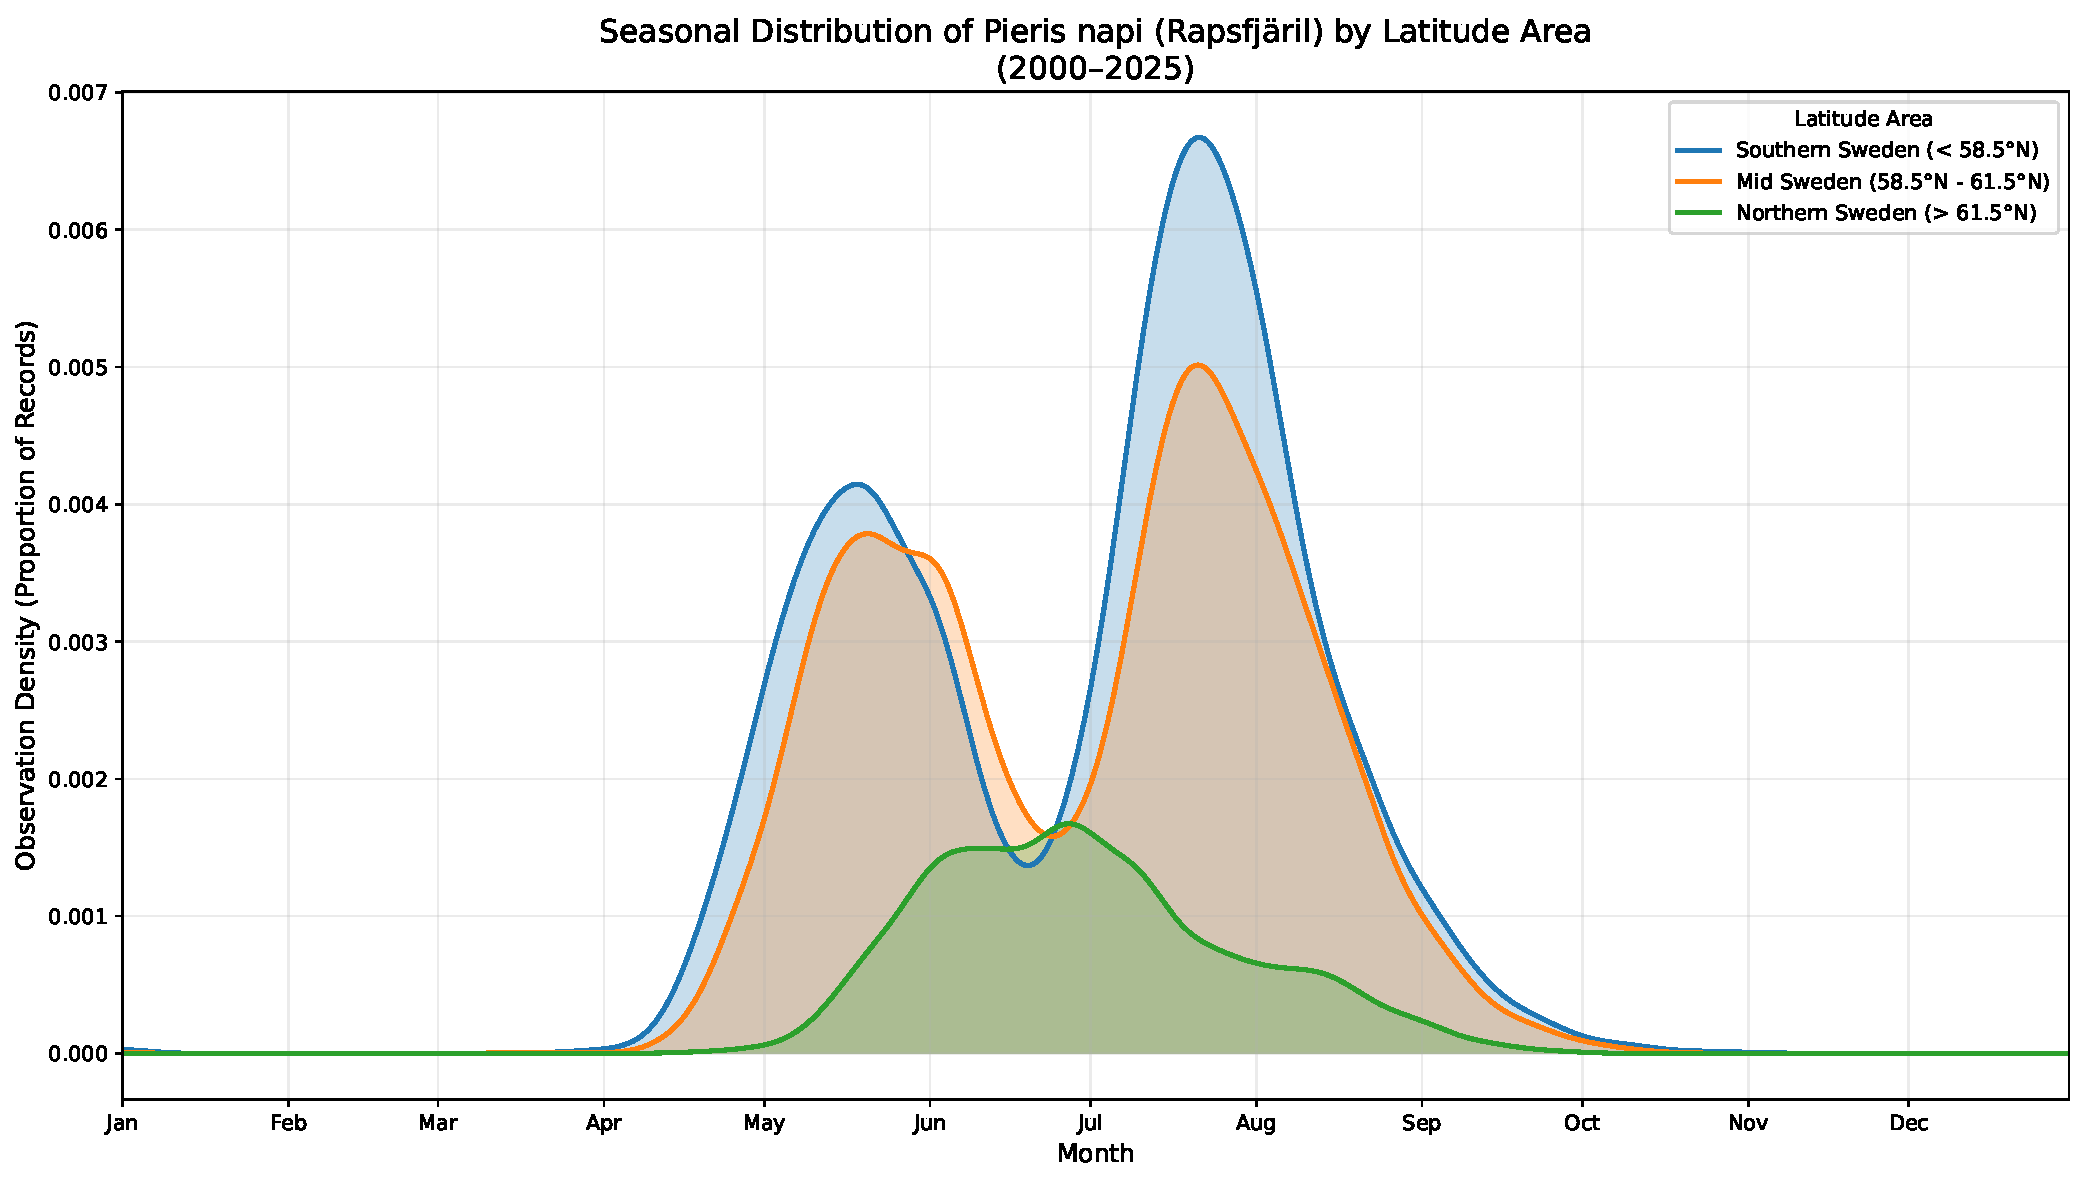
\includegraphics[width=1.3\textwidth]{figures/Pieris_napi_latitude_density.pdf}}

    \caption{Seasonal distribution of observations across three latitude areas in Sweden (2000--2025) for \textit{Pieris rapae} and \textit{Pieris napi}.}
    
    \label{fig:latitude-species}
\end{figure}

\FloatBarrier % stops figures from drifting into the discussion

\begin{figure}[!htb]
    \centering
    \makebox[\textwidth][c]{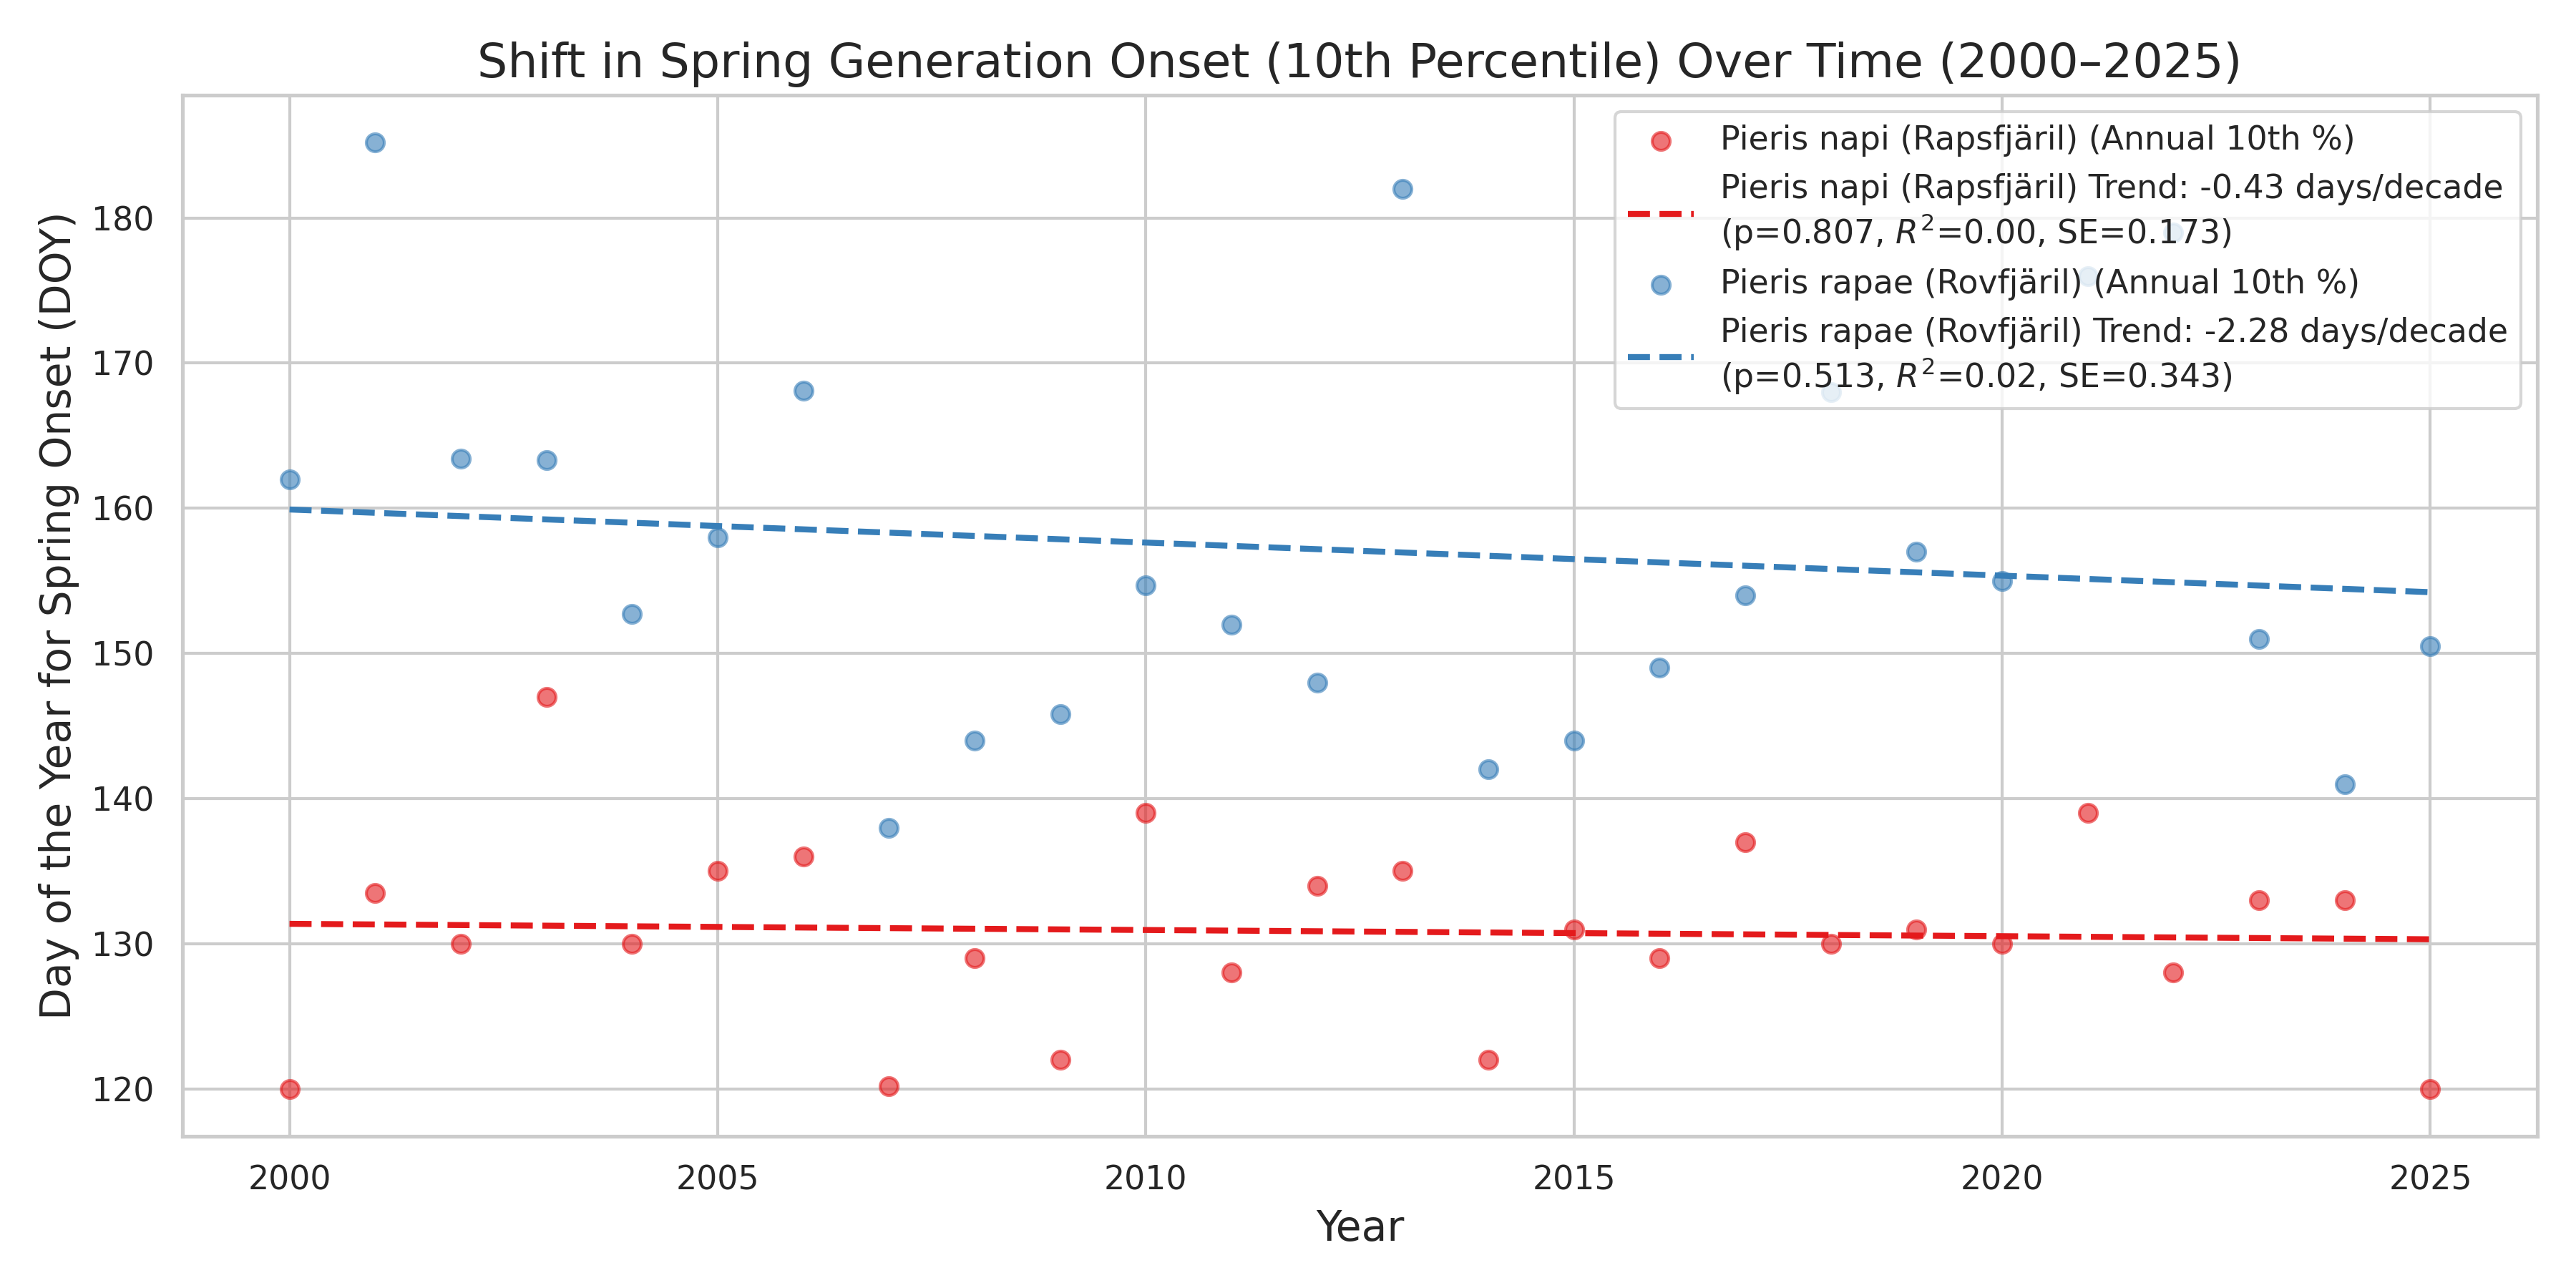
\includegraphics[width=1.3\textwidth]{figures/figure_3_climate_trend.png}}
    \caption{Long-term shift in the onset of the spring generation for Pieris napi and Pieris rapae in Sweden (2000–2025). The onset of the spring flight period is defined as the annual 10th percentile of the day of the year (DOY) for adult observations to minimize the influence of early outliers. Points represent annual calculated thresholds, and dashed lines indicate ordinary least squares (OLS) linear regressions. Statistical summaries, including the trend slope (days/decade), standard error (SE), coefficient of determination ($R^2$), and significance level ($p$), are displayed in the legend.}
    \label{fig:climate_trend}
\end{figure}

\begin{figure}[!htb]
    \centering
    \makebox[\textwidth][c]{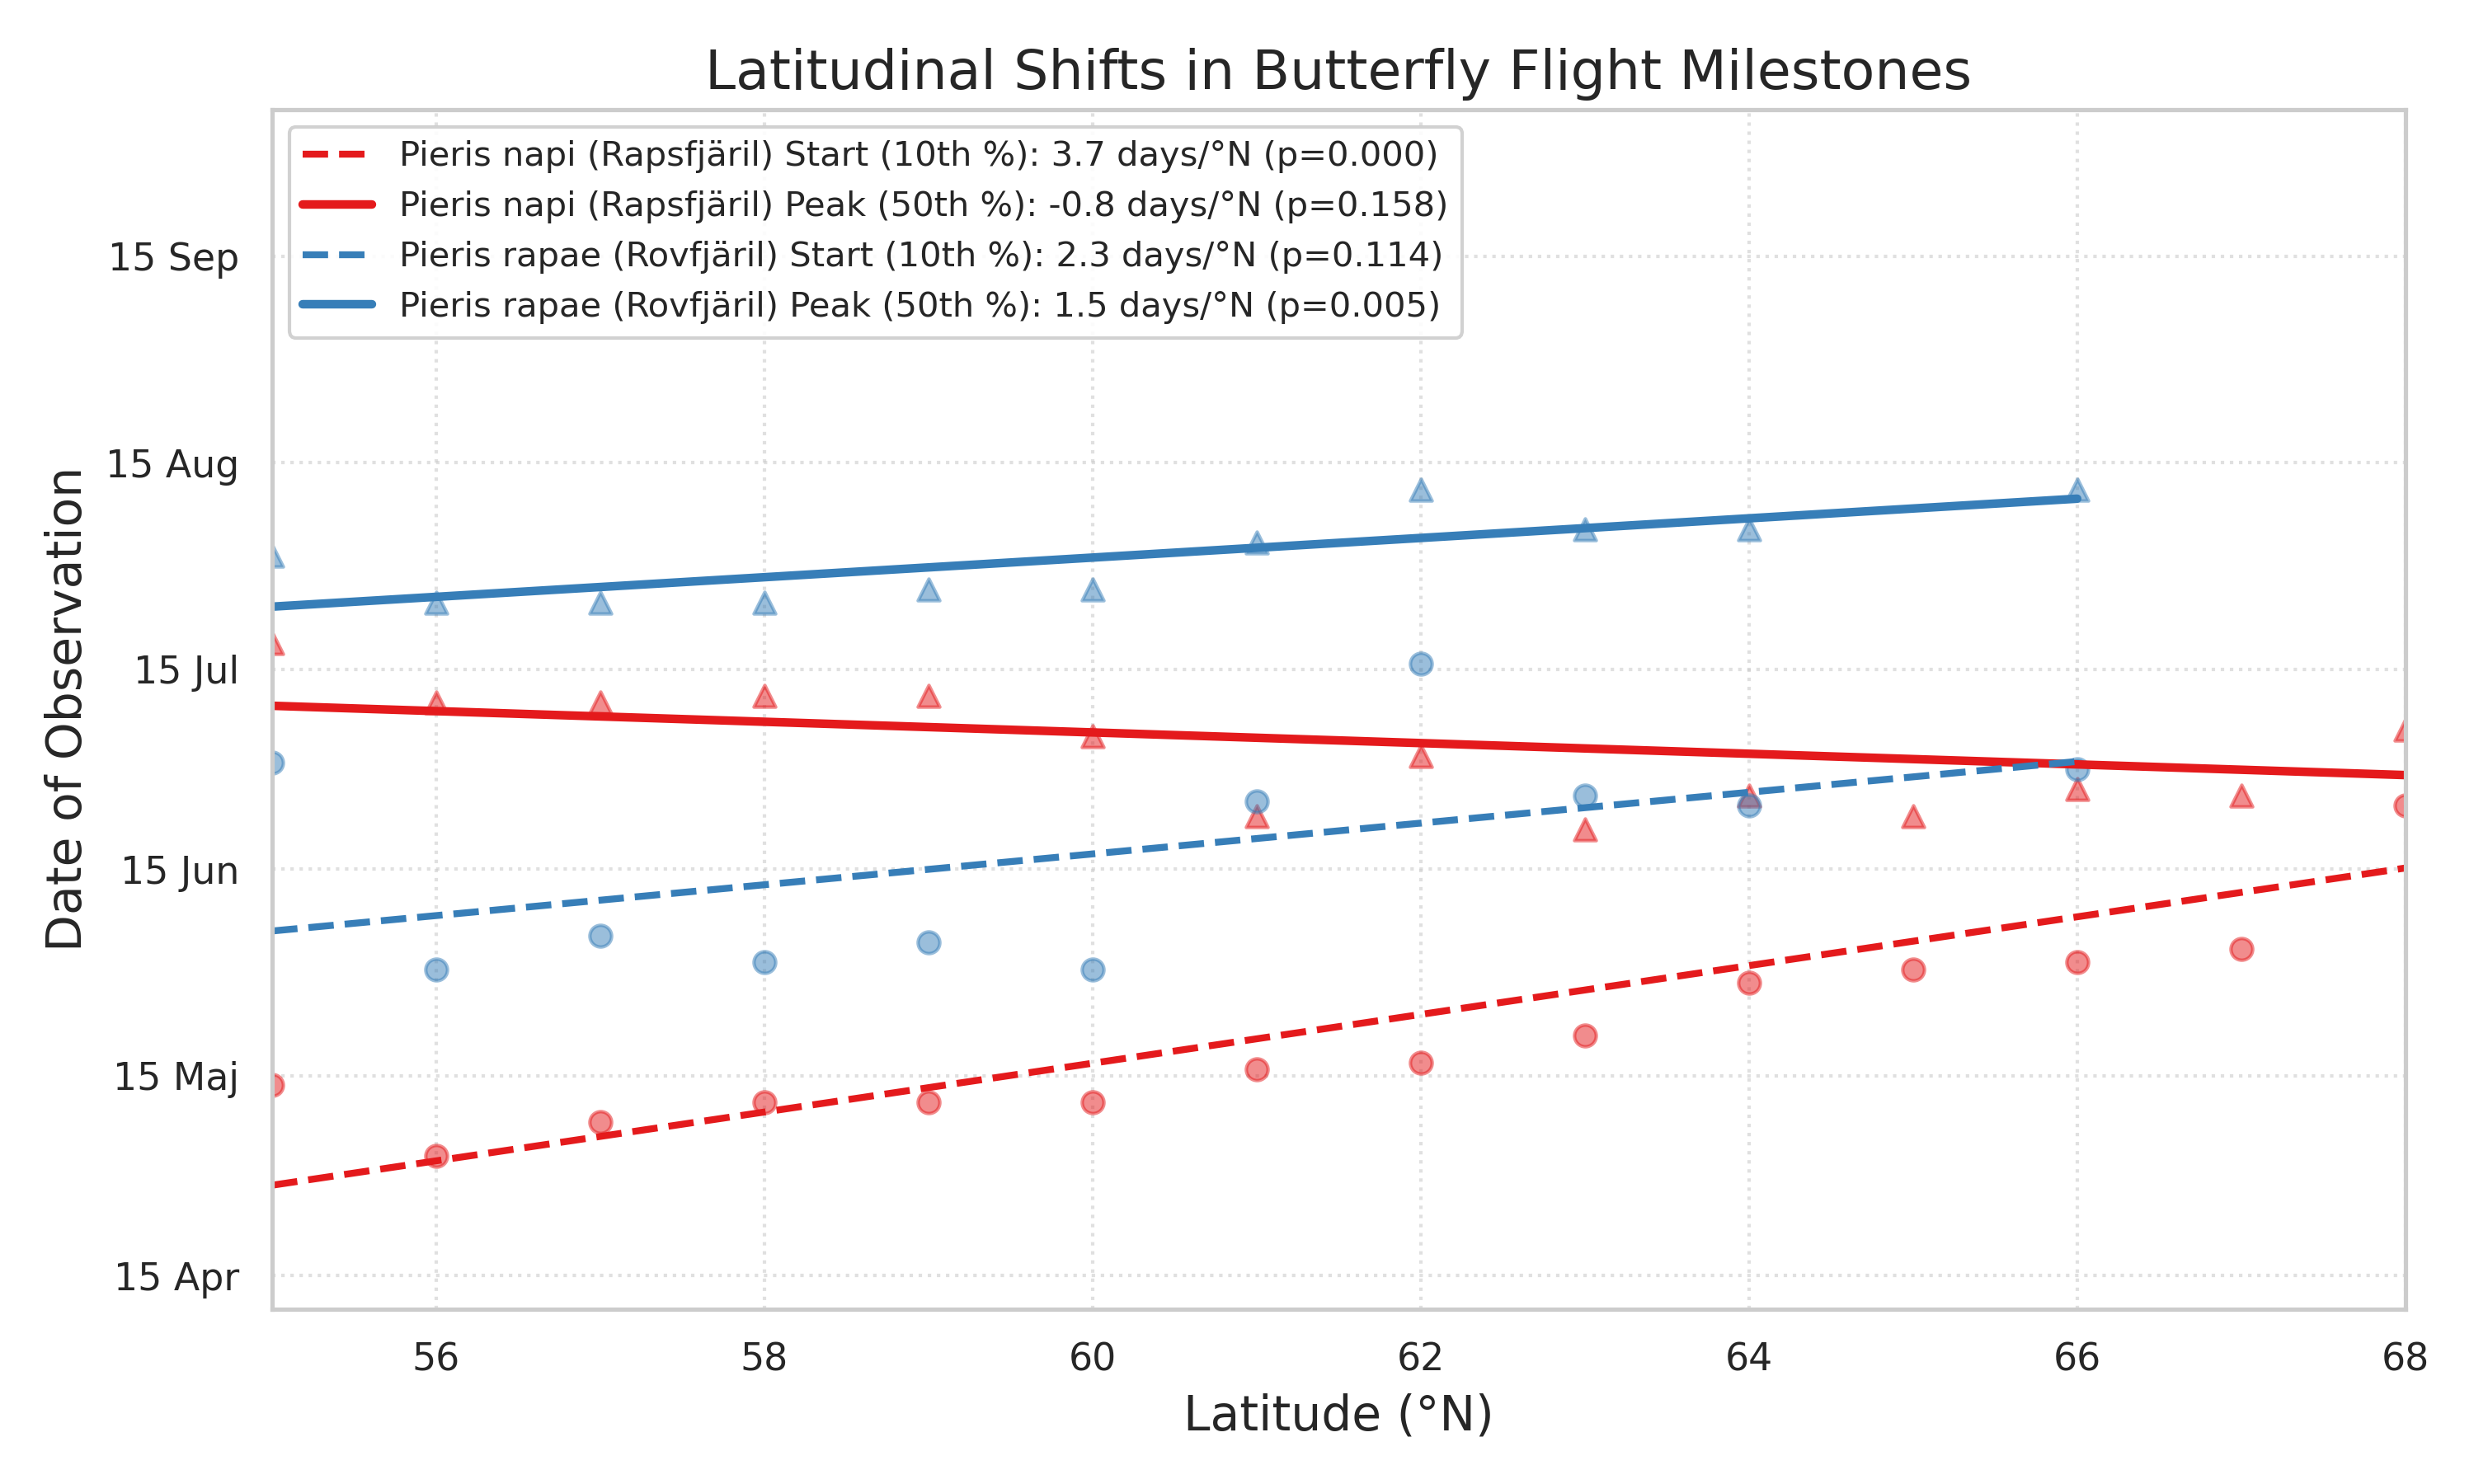
\includegraphics[width=1.4\textwidth]{figures/figure_4_latitude_gradient.png}}
    \caption{Latitudinal shifts in flight milestones for \textit{Pieris napi} and \textit{Pieris rapae} across Sweden (2000--2025). The graph groups observations by latitude degrees to show the spring start (10th percentile, dashed lines) and peak flight time (50th percentile/median, solid lines) for each species. The trend lines show how many days later these milestones occur for every degree North we move.}
    \label{fig:latitude_gradient}
\end{figure}

\FloatBarrier

\section{Discussion}

In Figure~\ref{fig:seasonal_phenology} we note that the two prominent peaks represent the spring (first) and summer (second) generations, demonstrating a characteristic bivoltine life cycle for both species. We can additionally see from the figure that \textit{P. napi} generally fare better at surviving the winter as pupae and hatching in April-May. After this follows a decrease in the number of individuals, as most of the spring generation of butterflies die before the summer generation has hatched. However, when the summer generation pupae hatch we can note that there are more hatched \textit{P. rapae}. 

From Figure~\ref{fig:latitude_effect} we note that the KDE distributions show a transition from a highly distinct bivoltine pattern (two separate peaks) in the south to a protracted, single-peak (univoltine) distribution in the north, illustrating latitudinal constraints on the development of a second summer generation.

The figures \ref{fig:latitude-species} show clear seasonal differences in the distribution of observations across latitude areas. For \textit{Pieris napi}, southern and mid Sweden show two main peaks, one during late spring/early summer and a second, larger peak during July, suggesting the occurrence of approximately two generations. A weaker and broader pattern is observed in northern Sweden, where the shorter growing season may result in fewer generations. For \textit{Pieris rapae}, the observations are mainly concentrated in southern and mid Sweden, with a smaller early-season peak followed by a pronounced peak in July--August, also suggesting approximately two generations. The northern \textit{P. rapae} curve is almost absent because very few observations were recorded above $61.5^\circ$N, making it difficult to draw reliable conclusions about its generational pattern there. Overall, the figures suggest that both species have multiple generations during the warmer months, while the number and strength of seasonal peaks tend to decrease towards higher latitudes.

As shown in Figure~\ref{fig:climate_trend}, the spring onset dates show a very slight shift of $-2.28$ days per decade for \textit{Pieris rapae} and $-0.43$ days per decade for \textit{Pieris napi}. However, neither trend is statistically reliable; the high $p$-values ($p = 0.51$ for \textit{P. rapae} and $p = 0.81$ for \textit{P. napi}) and $R^2$ values near zero show that the passing of years does not explain when the butterflies emerge. Instead, the start dates fluctuate heavily from year to year, driven by short-term weather rather than a steady climate trend. Despite this lack of a long-term trend, a highly consistent difference remains between the two species: \textit{P. napi} consistently emerges about two to three weeks earlier in the spring than \textit{P. rapae} every single year. This seems to strengthen the theory that \textit{P. napi} is better adapted to the cold. 

Additionally, the magnitude of this year-to-year variation is visibly more pronounced for \textit{P. rapae} than for \textit{P. napi}. \textit{P. napi's} spring onset dates are relatively tightly clustered within a narrower window, whereas \textit{P. rapae's} onset dates show a much wider annual spread. 

This pattern suggests that \textit{P. rapae} may be more sensitive to annual temperature and weather fluctuations than \textit{P. napi}. In harmony with our previous observations, \textit{P. napi} is less affected by the cold and therefore can have a more stable, cold-tolerance spring emergence, whereas \textit{P. rapae's} spring flight is much more vulnerable to unpredictable Swedish spring weather.

As shown in figure~\ref{fig:latitude_gradient}, we can observe two distinct geographical patterns in the milestone data. For \textit{Pieris rapae}, both the spring start and peak flight dates increase steadily as we move north, but all observations for this species stop entirely at latitude 66$^\circ$N. In contrast, the start and peak trendlines for \textit{Pieris napi} converge at higher latitudes, and its observations continue further north up to latitude 68$^\circ$N. This narrowing gap shows that the time window between the first spring emergence and peak activity shrinks significantly in colder northern climates, whereas \textit{P. rapae} is simply not recorded in these northernmost regions of Sweden.

\pagebreak
\printbibliography
\end{document}